\documentclass{article}
\usepackage{fontspec, xunicode, xltxtra} 
\setmainfont{Microsoft YaHei} 
\usepackage{setspace}
\usepackage{ctex} 
\usepackage{geometry}
\usepackage[Glenn]{fncychap}
\usepackage{listings}
\usepackage{color}
\usepackage{verbatim}
\usepackage{fancyhdr}
\usepackage{graphicx}


\newfontfamily\monaco{Monaco}
%\hspace{2em plus 1em minus 0.25em}

%\title{靠别人,你永远是右倾投降主义\\靠自己,你才是工农武装割据}
%\author{ZJUT14}

\definecolor{dkgreen}{rgb}{0,0.6,0}
\definecolor{gray}{rgb}{0.5,0.5,0.5}
\definecolor{mauve}{rgb}{0.58,0,0.82}

\geometry{left=2cm,right=1.7cm,top=2cm,bottom=1.7cm}
%\rhead{\CJKfamily{kai} 第 \thepage 页}
%\lfoot{} 
%\cfoot{\thepage}
%\rfoot{}
%\newcommand{\makefirstpageheadrule}{
%\makebox[0pt][l]{\rule[0.55\baselineskip]{\headwidth}{0.4pt}}
%\rule[0.7\baselineskip]{\headwidth}{0.4pt}}

%\renewcommand{\footrulewidth}{0.2pt}
\setlength{\skip\footins}{0.3cm}

\lstset{
    frame=simple,
    language=  c++,
    aboveskip=3mm,
    belowskip=3mm,
    showstringspaces=false,
    basicstyle=\small\monaco,
    numbers=none,
    numberstyle=\tiny\color{gray},
    keywordstyle=\bfseries\monaco,%\fontspec{monaco Bold}\bfseries,
    commentstyle=\color{dkgreen},
    stringstyle=\color{mauve},
    breaklines=true,
    breakatwhitespace=true,
    tabsize=4,
    numbers = left,
    numberstyle=\tiny\monaco,
}

\begin{document}

\begin{titlepage}

\thispagestyle{empty}
\pagebreak
\textbf{其它}
\pagestyle{plain}
\tableofcontents



\hspace{3em}
\section{快读}
\lstinputlisting{快读.cpp}
%\section{__int128}
%\lstinputlisting{__int128.cpp}
\section{对拍}
\lstinputlisting{对拍.cpp}
\section{华容道}
\lstinputlisting{华容道.cpp}
\section{希尔伯特曲线}
\begin{figure}[htb] 
 \center{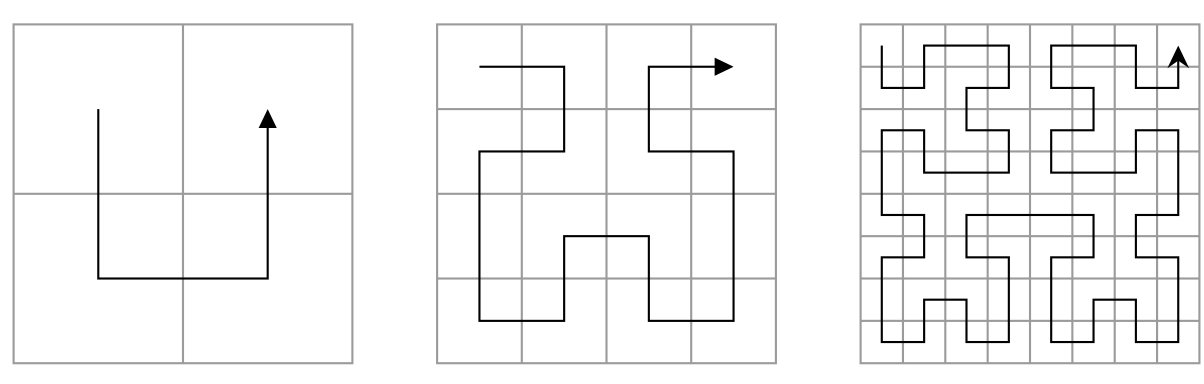
\includegraphics[width=15cm]  {希尔伯特曲线_pic.png}} 
 \end{figure}
\lstinputlisting{希尔伯特曲线.cpp}
\section{约瑟夫环}
\subsection{一般方法}
\lstinputlisting{约瑟夫环/一般方法.cpp}
\subsection{函数图像解}
\lstinputlisting{约瑟夫环/函数图像解.cpp}

\end{titlepage}

\end{document}